\addchap{Anhang}

\section*{TEIL A: Autoren der einzelnen Kapitel}
Auf den folgenden Seiten werden die Kapitel in den Farben der Autoren markiert.
Dabei steht die Farbe blau für \daniel{Daniel Brown}, grün für \jani{Jan-Eric Gaidusch} und gelb für \samuel{Samuel Philipp}.

\rule{\textwidth}{1pt}

\daniel{Abstract}

{1 Einleitung}

\samuel{1.1 Einf\"uhrung}

\jani{1.2 Hintergrund}

\samuel{1.3 Aufgabenstellung}

\daniel{1.4 Team}

\samuel{1.5 webifier}

{2 Grundlagen}

\daniel{2.1 Frontend Technologien und Framework}

{2.2 Backend Technologien und Frameworks}

\indent \samuel{- Java}

\indent \samuel{- Spring}

\indent \samuel{- MongoDB}

\indent \jani{- Gradle}

\indent \jani{- Rest}

\indent \jani{- Docker}

\indent \jani{- R}

{2.3 Technologien und Frameworks der Tests}

\indent \daniel{- Python}

\indent \daniel{- PhantomJS}

\indent \jani{- Bro}

\indent \samuel{- HTtrack}

\indent \samuel{- Resemble.js}

{2.4 Angriffstypen}

\samuel{2.4.1 Malware}

\daniel{2.4.2 Request Header Investigation}

\jani{2.4.3 JavaScript Port \& IP Scanning}

\samuel{2.4.4 Phishing}

{3 Konzept}

{3.1 Gesamtkonzept}

\jani{3.1.1 webifier Tests}

\samuel{3.1.2 webifier Tester}

\samuel{3.1.3 webifier Platform}

\daniel{3.1.4 webifier Mail}

\samuel{3.1.5 webifier Data}

\jani{3.1.6 webifier Statistics}

{3.2 Testarten}

\samuel{3.2.1 Virenscan}

\daniel{3.2.2 Vergleich in verschiedenen Browsern}

\jani{3.2.3 Test auf Port Scanning}

\jani{3.2.4 Test auf IP Scanning}

\daniel{3.2.5 Link Checker}

\daniel{3.2.6 Google Safe Browsing}

\samuel{3.2.7 \"Uberpr\"ufung des Zertifikats}

\samuel{3.2.8 Erkennung von Phishing}

\jani{3.2.9 Screenshot}

{4 Umsetzung}

{4.1 Gesamtanwendung}

\jani{4.1.1 webifier Tests}

\samuel{4.1.2 webifier Tester}

\samuel{4.1.3 webifier Platform}

\daniel{4.1.4 webifier Mail}

\samuel{4.1.5 webifier Data}

\jani{4.1.6 webifier Statistics}

{4.2 Tests}

\samuel{3.2.1 Virenscan}

\daniel{3.2.2 Vergleich in verschiedenen Browsern}

\jani{4.2.3 Test auf Port Scanning}

\jani{4.2.4 Test auf IP Scanning}

\daniel{4.2.5 Link Checker}

\daniel{4.2.6 Google Safe Browsing}

\samuel{4.2.7 \"Uberpr\"ufung des Zertifikats}

\samuel{4.2.8 Erkennung von Phishing}

\jani{4.2.9 Screenshot}

{5 Analyse}

{6 Ausblick}

{6.1 Weitere Tests}

{6.2 Weitere Module}

{7 Fazit}

{7.1 Zusammenfassung}

{7.2 Bewertung der Ergebnisse}

\newpage

\section*{TEIL B: Vollständige Konfigurationsdatei webifier Tester}
\label{app:b}

\begin{scriptsize}
\lstset{
    style=eclipsejavascript,
    caption={Vollständige Konfigurationsdatei webifier Tester}
}
\begin{lstlisting}
{
  "resolver": {
    "name": "resolver",
    "startup": "docker run --rm --name #ID -e URL=#URL -e ID=#ID webifier-resolver",
    "startup_timeout_seconds": 60,
    "shutdown": "docker stop #ID",
    "shutdown_timeout_seconds": 30
  },
  "tests": [
    {
      "name": "VirusScan",
      "startup": "docker run --rm --name #ID -e URL=#URL -e ID=#ID webifier-test-virusscan",
      "startup_timeout_seconds": 600,
      "shutdown": "docker stop #ID",
      "shutdown_timeout_seconds": 30,
      "result_class": "de.securitysquad.webifier.output.result.virusscan.TestVirusScanResultInfo",
      "weight": 5,
      "enabled": true
    },
    {
      "name": "HeaderInspection",
      "startup": "docker run --rm --name #ID -e URL=#URL -e ID=#ID webifier-test-header-inspection",
      "startup_timeout_seconds": 300,
      "shutdown": "docker stop #ID",
      "shutdown_timeout_seconds": 30,
      "result_class": "de.securitysquad.webifier.output.result.headerinspection.HeaderInspectionResultInfo",
      "weight": 1,
      "enabled": true
    },
    {
      "name": "PortScan",
      "startup": "docker run --rm --name #ID -e URL=#URL -e ID=#ID webifier-test-portscan",
      "startup_timeout_seconds": 300,
      "shutdown": "docker stop #ID",
      "shutdown_timeout_seconds": 30,
      "result_class": "de.securitysquad.webifier.output.result.portscan.TestPortScanResultInfo",
      "weight": 3,
      "enabled": true
    },
    {
      "name": "IpScan",
      "startup": "docker run --rm --name #ID -e URL=#URL -e ID=#ID webifier-test-ipscan",
      "startup_timeout_seconds": 300,
      "shutdown": "docker stop #ID",
      "shutdown_timeout_seconds": 30,
      "result_class": "de.securitysquad.webifier.output.result.ipscan.TestIpScanResultInfo",
      "weight": 3,
      "enabled": true
    },
    {
      "name": "Screenshot",
      "startup": "docker run --rm --name #ID -e URL=#URL -e ID=#ID webifier-test-screenshot",
      "startup_timeout_seconds": 300,
      "shutdown": "docker stop #ID",
      "shutdown_timeout_seconds": 30,
      "result_class": "de.securitysquad.webifier.output.result.screenshot.TestScreenshotResultInfo",
      "weight": 0,
      "enabled": true
    },
    {
      "name": "LinkChecker",
      "startup": "docker run --rm --name #ID -e URL=#URL -e ID=#ID webifier-test-linkchecker",
      "startup_timeout_seconds": 300,
      "shutdown": "docker stop #ID",
      "shutdown_timeout_seconds": 30,
      "result_class": "de.securitysquad.webifier.output.result.linkchecker.TestLinkCheckerResultInfo",
      "weight": 1,
      "enabled": true
    },
    {
      "name": "CertificateChecker",
      "startup": "docker run --rm --name #ID -e URL=#URL -e ID=#ID webifier-test-certificatechecker",
      "startup_timeout_seconds": 300,
      "shutdown": "docker stop #ID",
      "shutdown_timeout_seconds": 30,
      "result_class": "de.securitysquad.webifier.output.result.certificatechecker.TestCertificateCheckerResultInfo",
      "weight": 3,
      "enabled": true
    },
    {
      "name": "PhishingDetector",
      "startup": "docker run --rm --name #ID -e URL=#URL -e ID=#ID webifier-test-phishingdetector",
      "startup_timeout_seconds": 300,
      "shutdown": "docker stop #ID",
      "shutdown_timeout_seconds": 30,
      "result_class": "de.securitysquad.webifier.output.result.phishingdetector.TestPhishingDetectorResultInfo",
      "weight": 5,
      "enabled": true
    },
    {
      "name": "GoogleSafeBrowsing",
      "startup": "docker run --rm --name #ID -e URL=#URL -e ID=#ID -e API_KEY=INSERT_API_KEY webifier-test-google-safe-browsing",
      "startup_timeout_seconds": 300,
      "shutdown": "docker stop #ID",
      "shutdown_timeout_seconds": 30,
      "result_class": "de.securitysquad.webifier.output.result.googlesafebrowsing.TestGoogleSafeBrowsingResultInfo",
      "weight": 3,
      "enabled": true
    }
  ],
  "preferences": {
    "push_result_data": true
  }
}
\end{lstlisting}
\end{scriptsize}

\newpage

\section*{TEIL C: Vollständige Ergebnisberechnung webifier Tester}
\label{app:c}

\begin{scriptsize}
\lstset{
    style=eclipsejava,
    caption={Vollständige Ergebnisberechnung webifier Tester}
}
\begin{lstlisting}
private WebifierOverallTestResult calculateOverallResult() {
    int weightSum = #tests#.stream().map(WebifierTest::getData).mapToInt(WebifierTestData::getWeight).sum();
    int mostWeighted = #tests#.stream().map(WebifierTest::getData).mapToInt(WebifierTestData::getWeight).max().orElse(weightSum / 2);
    double maliciousMin = (double) mostWeighted / (double) weightSum;
    double suspiciousMin = Math.pow(maliciousMin, 2);

    int undefinedTestSum = #tests#.stream().filter(test -> test.getResult().getResultType() == WebifierResultType.##UNDEFINED##)
            .map(WebifierTest::getData).mapToInt(WebifierTestData::getWeight).sum();
    double undefinedPercentage = (double) undefinedTestSum / (double) weightSum;
    if (undefinedPercentage > #MAX_UNDEFINED_TEST_PERCENTAGE#) {
        return new WebifierOverallTestResult(WebifierResultType.##UNDEFINED##);
    }
    double result = 0;
    for (WebifierTest<TestResult> test : tests) {
        double testWeight = (double) test.getData().getWeight() / (double) weightSum;
        result += getTestResultValue(test.getResult().getResultType(), testWeight) * testWeight;
    }
    if (result >= maliciousMin) {
        return new WebifierOverallTestResult(WebifierResultType.##MALICIOUS##, result);
    }
    if (result >= suspiciousMin) {
        return new WebifierOverallTestResult(WebifierResultType.##SUSPICIOUS##, result);
    }
    return new WebifierOverallTestResult(WebifierResultType.##CLEAN##, result);
}

private double getTestResultValue(WebifierResultType type, double testWeight) {
    if (type == WebifierResultType.##MALICIOUS##) {
        return 1;
    }
    if (type == WebifierResultType.##SUSPICIOUS##) {
        return testWeight;
    }
    return 0;
}
\end{lstlisting}
\end{scriptsize}

\newpage


\begin{landscape}

\section*{TEIL D: webifier Platform - Screenshots}
\label{app:d}

\begin{figure}[H]
  \centering
  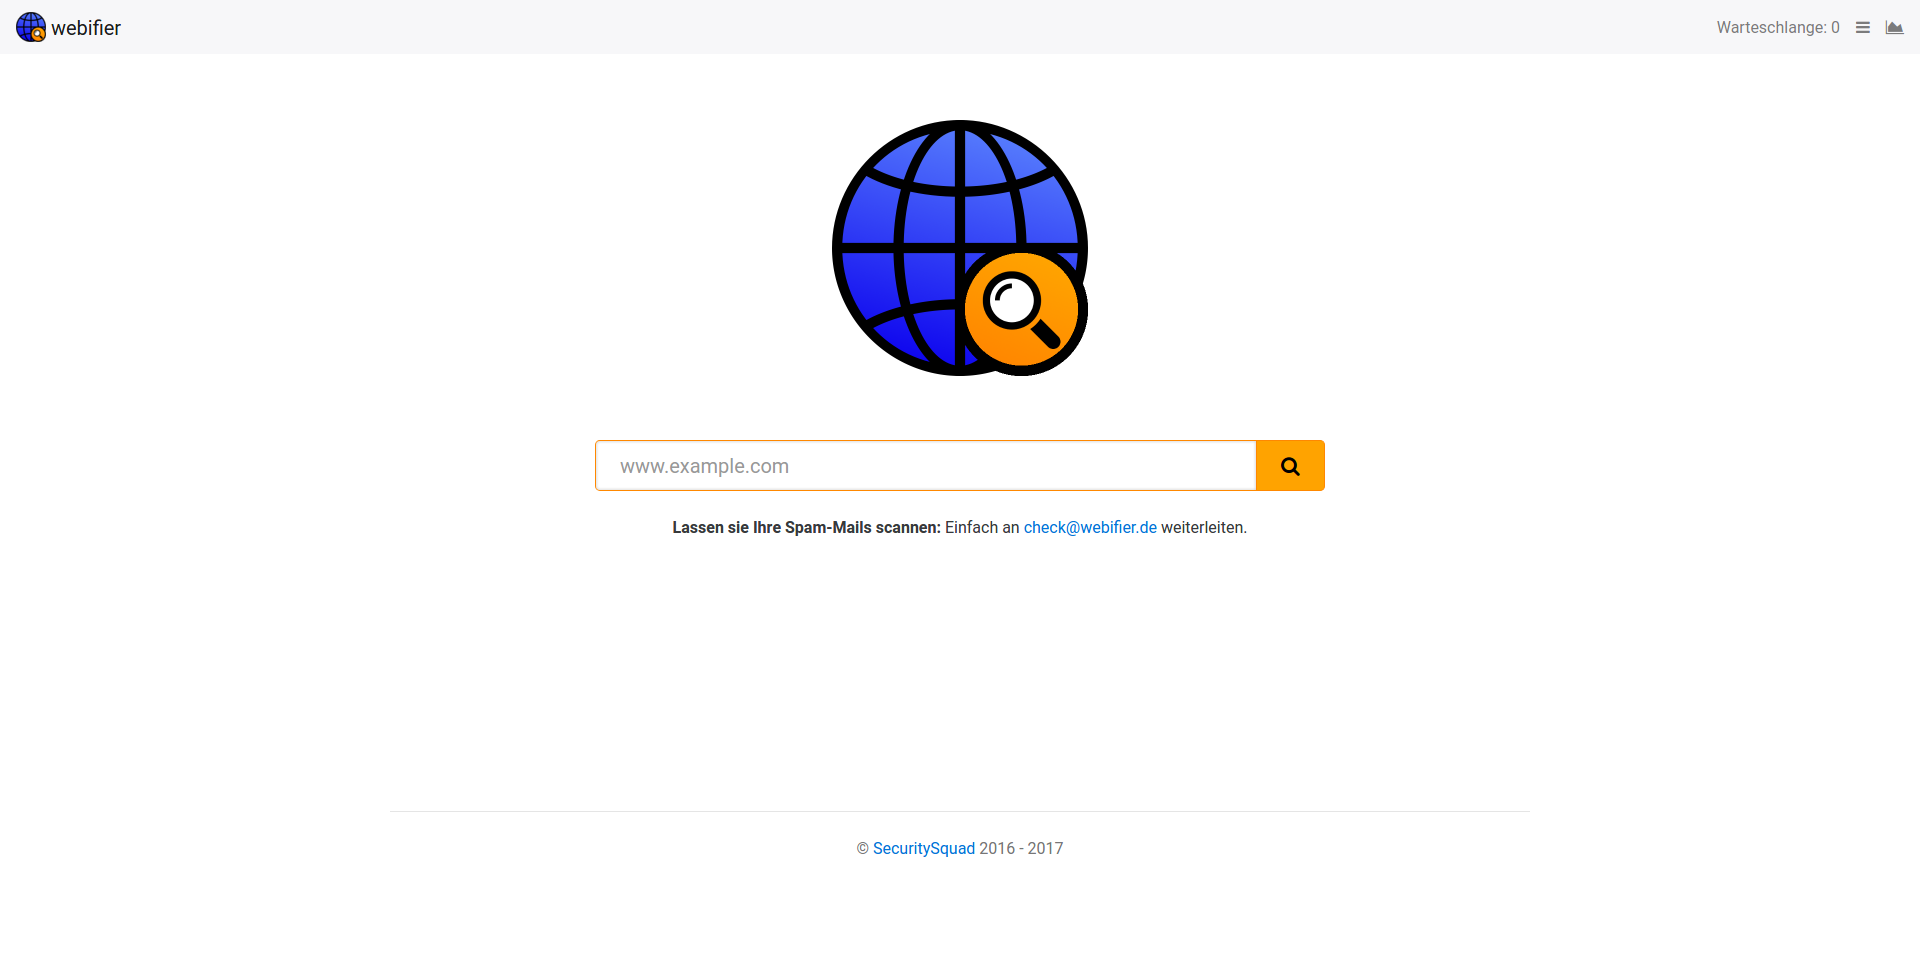
\includegraphics[width=\textheight]{images/platform/screenshot-start}
  \caption{webifier Platform - Startseite}
\end{figure}

\begin{figure}[H]
  \centering
  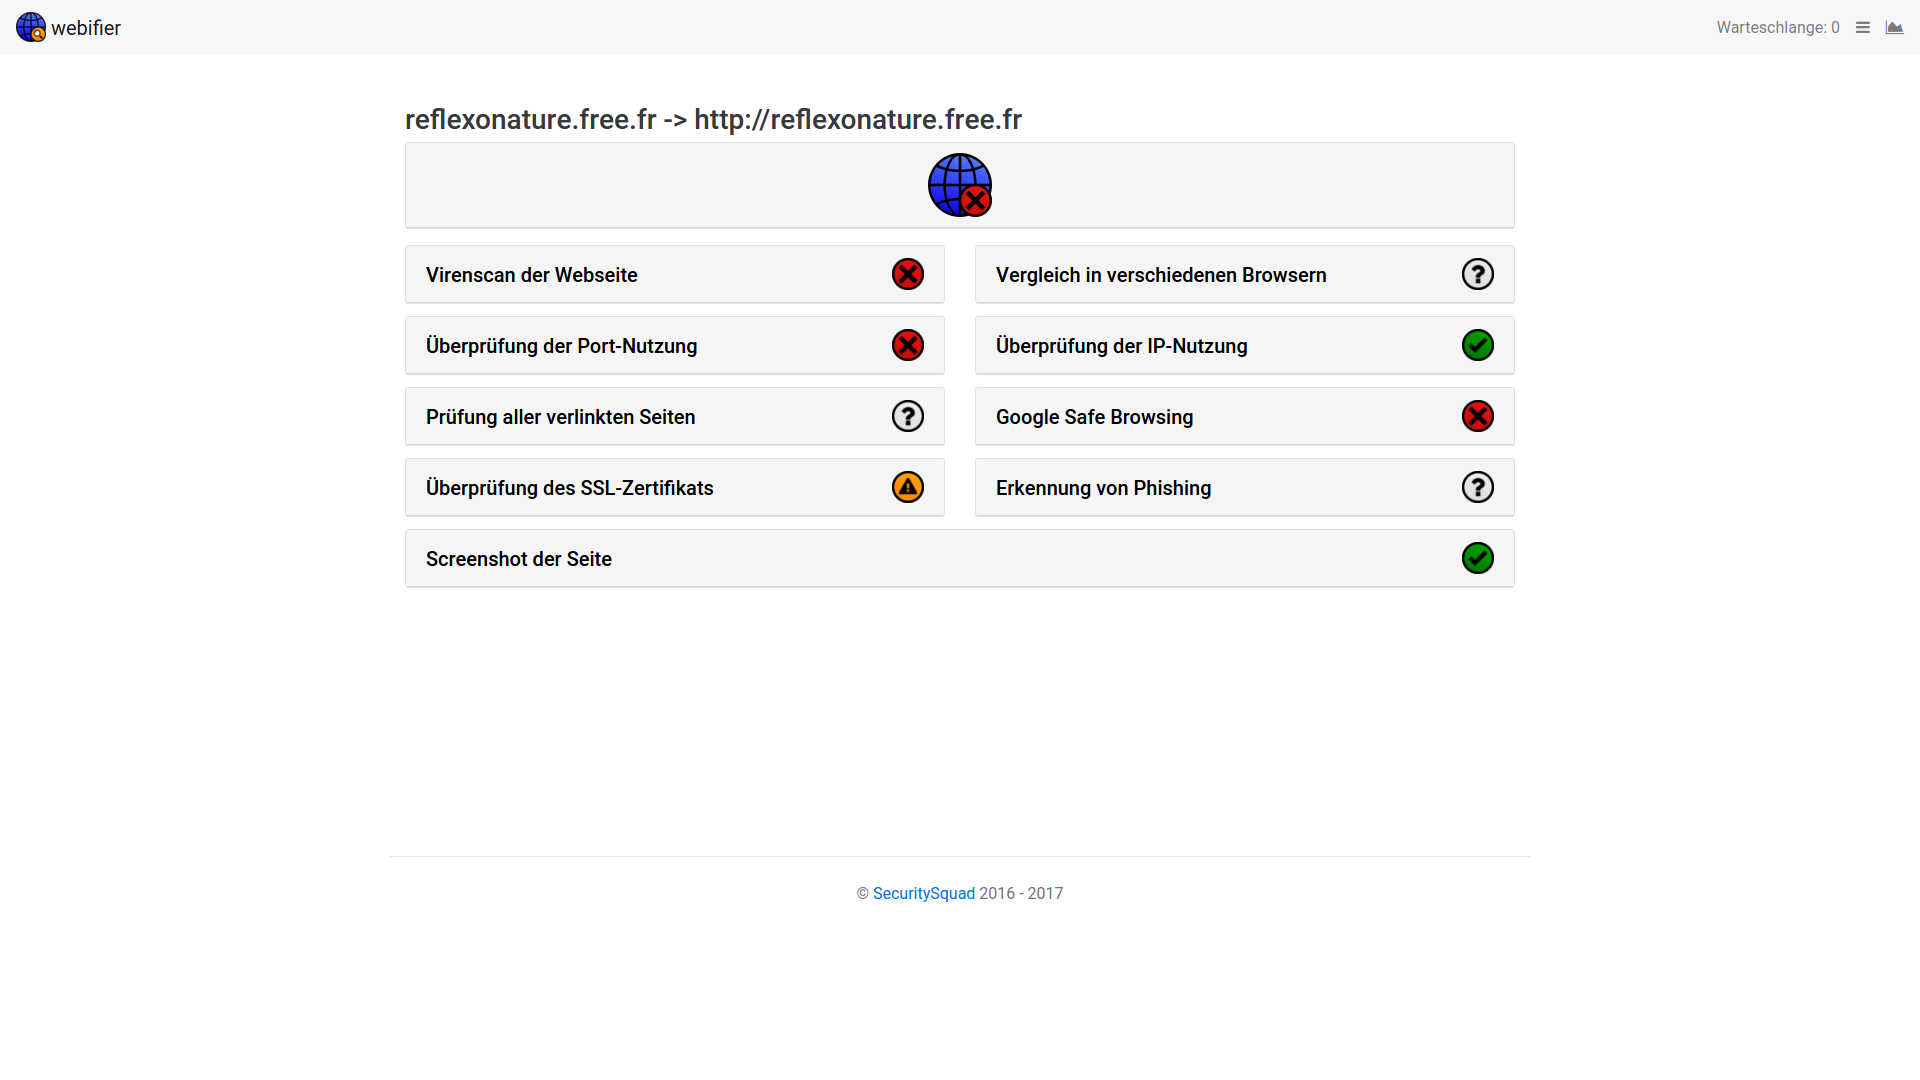
\includegraphics[width=\textheight]{images/platform/screenshot-reflexonature}
  \caption{webifier Platform - Ergebnisseite für reflexonature.free.fr}
  \label{fig:platform-result}
\end{figure}


\begin{figure}[H]
  \centering
  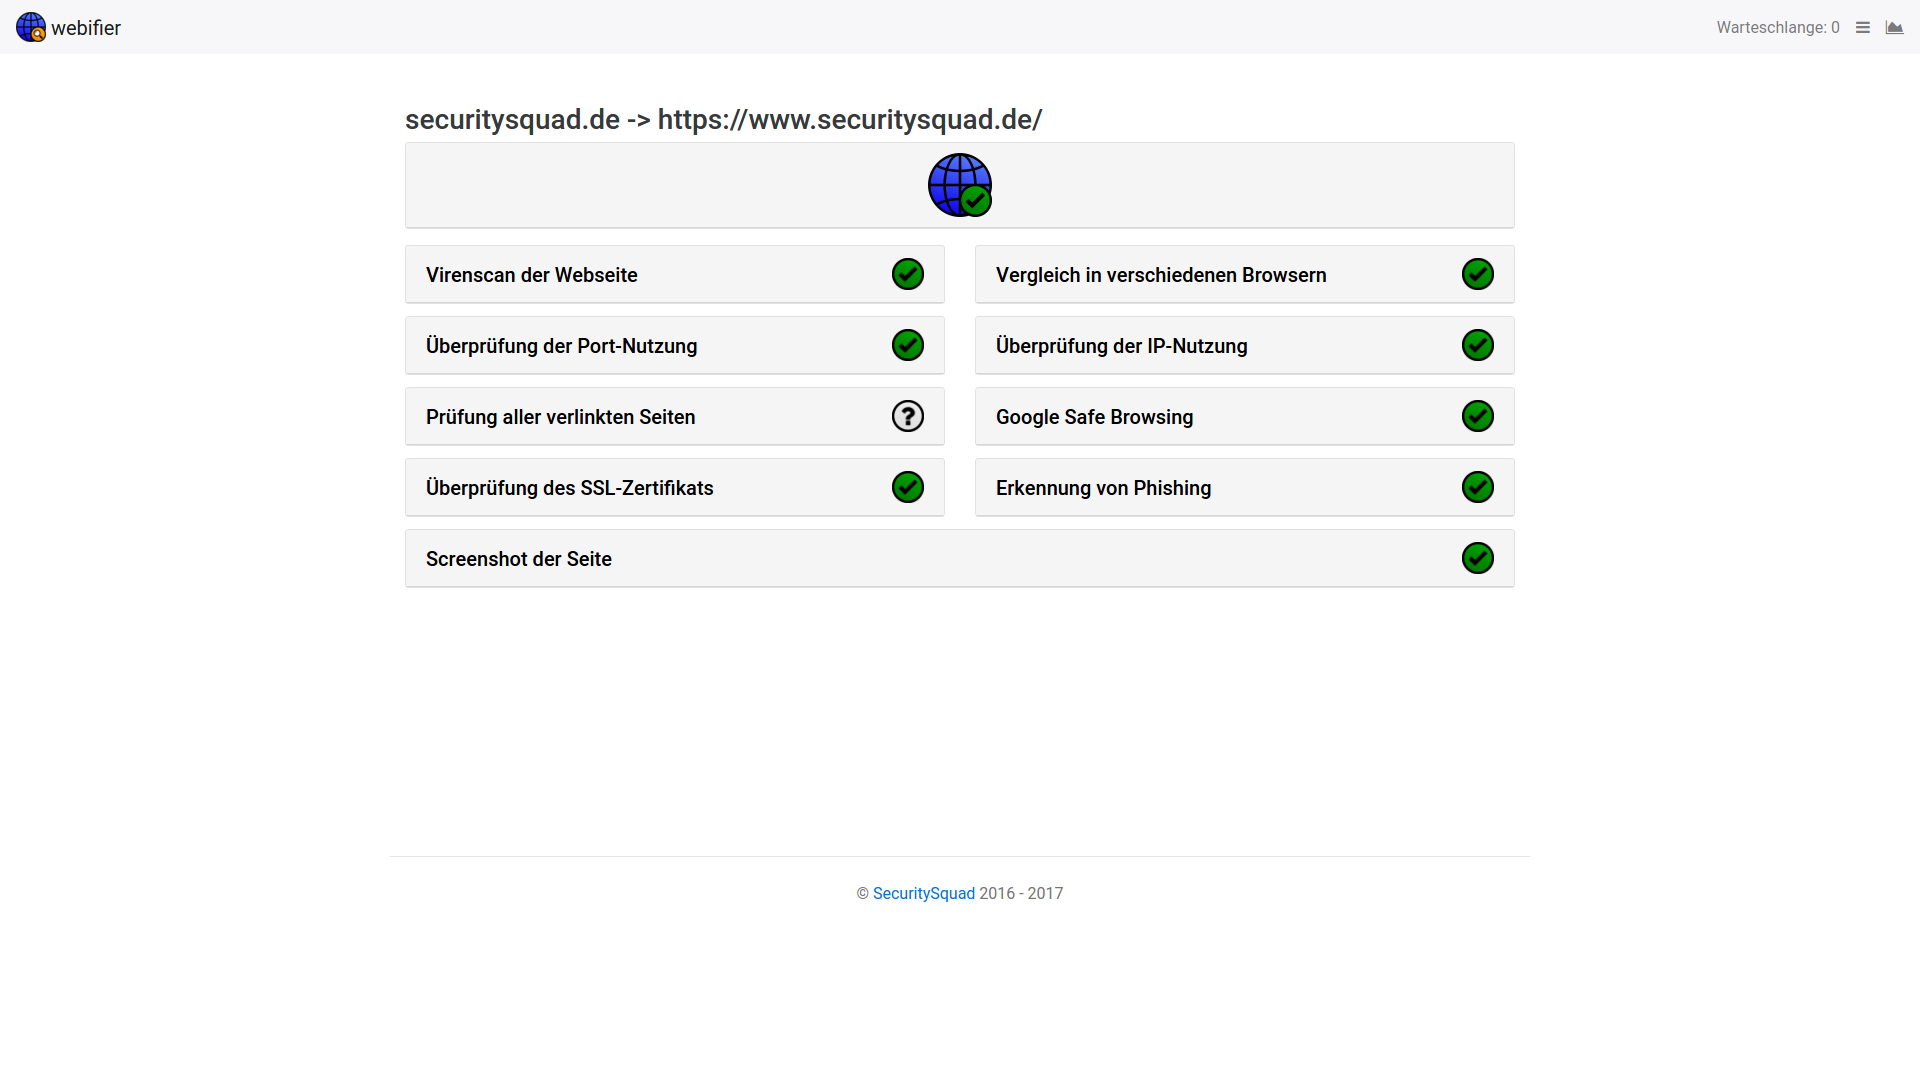
\includegraphics[width=\textheight]{images/platform/screenshot-securitysquad}
  \caption{webifier Platform - Ergebnisseite für securitysquad.de}
  \label{fig:platform-result}
\end{figure}


\begin{figure}[H]
  \centering
  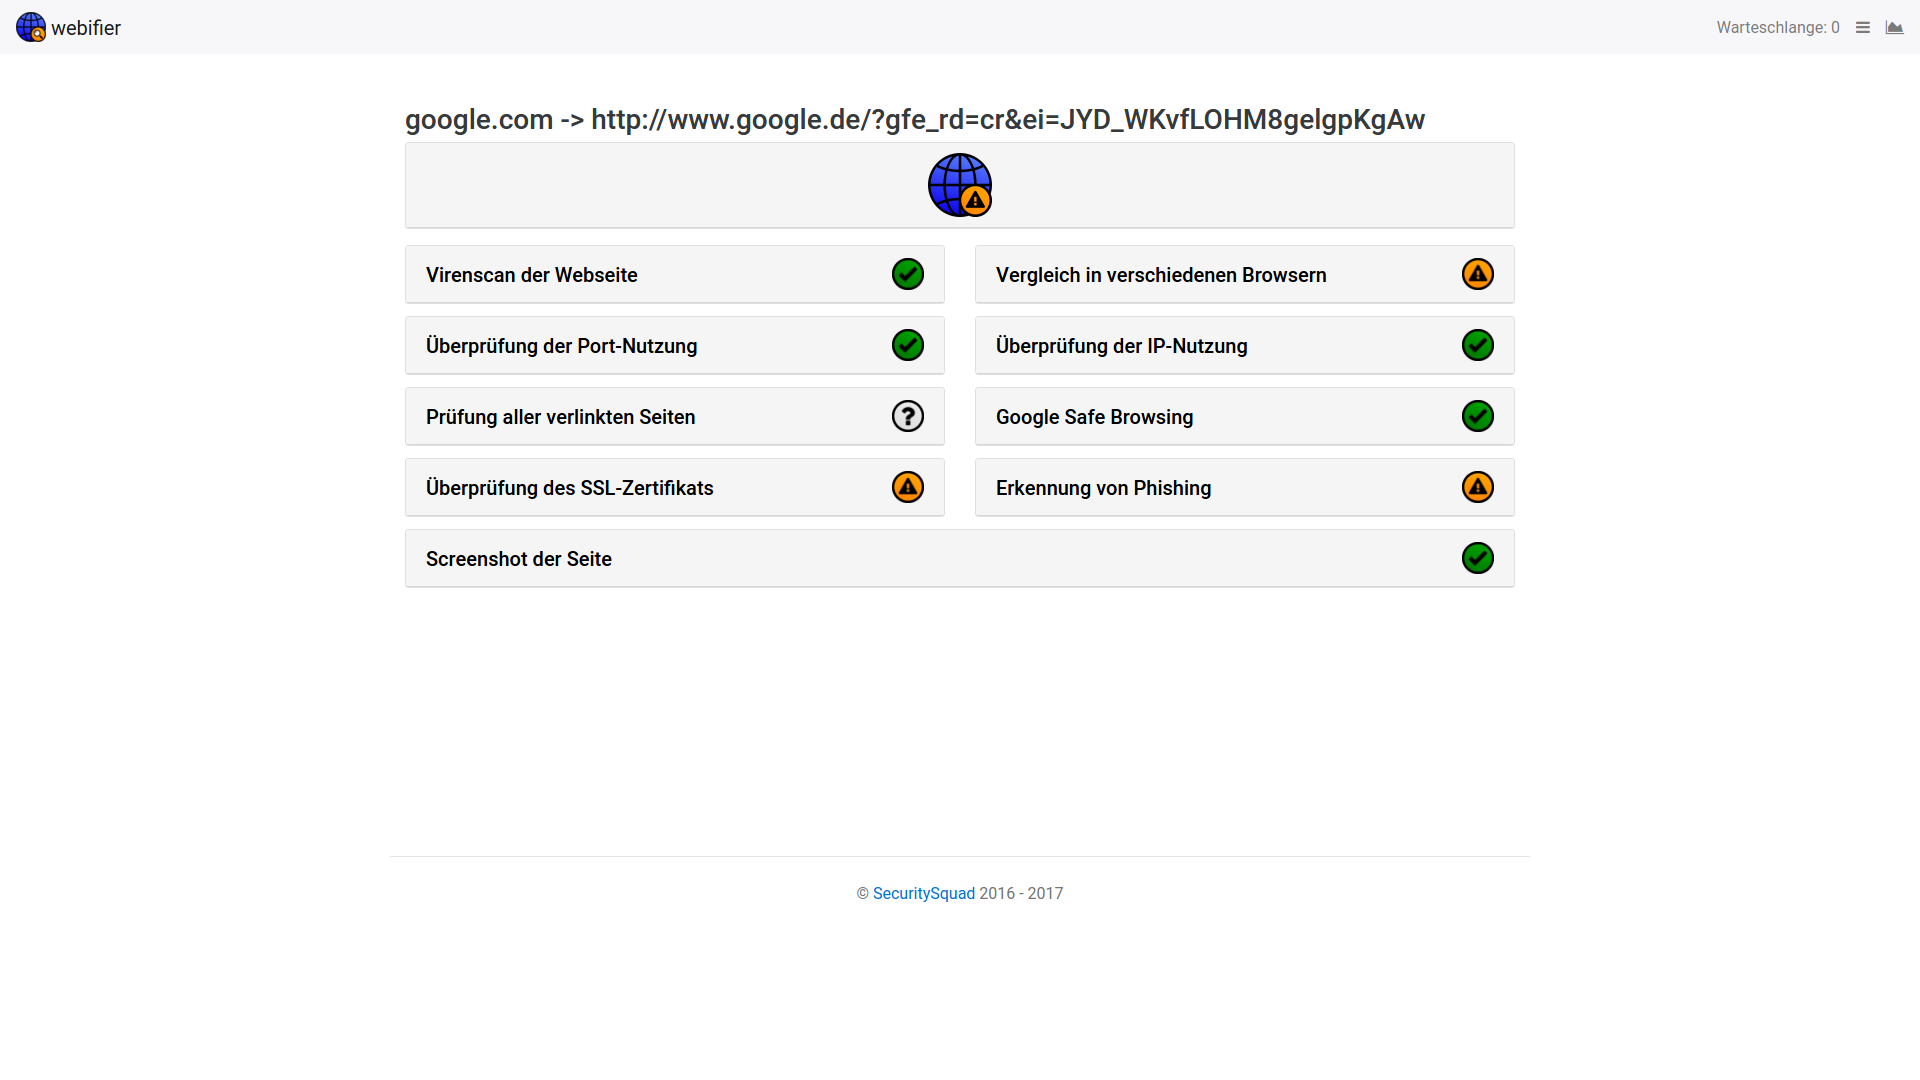
\includegraphics[width=\textheight]{images/platform/screenshot-google}
  \caption{webifier Platform - Ergebnisseite für google.com}
  \label{fig:platform-result}
\end{figure}


\end{landscape}

\newpage

\section*{TEIL E: Beispieldokumente webifierSingleTestResultData - webifier Data}
\label{app:e}

\begin{scriptsize}
\lstset{
    style=eclipsejavascript,
    caption={Beispieldokument webifierSingleTestResultData: Virenscan der Webseite - webifier Data},
}
\begin{lstlisting}
{
    "_id" : "2429f999-3168-4070-b085-7887ee64d8a0",
    "_class" : "de.securitysquad.webifier.persistence.domain.WebifierSingleTestResultData",
    "testId" : "61574eb4-e9ac-42e2-9140-4c1ce23a2891_5b8bcdbf-2d89-4930-915a-d65c5367bd28",
    "name" : "VirusScan",
    "startup" : "docker run --rm --name #ID -e URL=#URL -e ID=#ID webifier-test-virusscan",
    "shutdown" : "docker stop #ID",
    "enabled" : true,
    "weight" : 5,
    "startupTimeoutInSeconds" : 600,
    "shutdownTimeoutInSeconds" : 30,
    "result" : "MALICIOUS",
    "resultInfo" : {
        "scanned_files" : 4,
        "malicious_files" : 3,
        "suspicious_files" : 0,
        "files" : [
            {
                "name" : "index98e1.html",
                "result" : "MALICIOUS"
            },
            {
                "name" : "index-2.html",
                "result" : "CLEAN"
            },
            {
                "name" : "indexec9e.html",
                "result" : "MALICIOUS"
            },
            {
                "name" : "index3547.html",
                "result" : "MALICIOUS"
            }
        ]
    },
    "durationInMillis" : NumberLong(142805),
    "overallResult" : DBRef("webifierTestResultData", "82879e46-b286-4bdf-9876-875dc67e5708")
}
\end{lstlisting}
\end{scriptsize}

\newpage

\begin{scriptsize}
\lstset{
    style=eclipsejavascript,
    caption={Beispieldokument webifierSingleTestResultData: Vergleich in verschiedenen Browsern - webifier Data},
}
\begin{lstlisting}
{
    "_id" : "70210b9f-e4fc-475b-a40a-5c98f49a18d3",
    "_class" : "de.securitysquad.webifier.persistence.domain.WebifierSingleTestResultData",
    "testId" : "b19e3a9c-7bca-4d4f-b03b-a87e086d1592_2dd8aa86-b6b5-434a-a627-3ae11a0c1b9e",
    "name" : "HeaderInspection",
    "startup" : "docker run --rm --name #ID -e URL=#URL -e ID=#ID webifier-test-header-inspection",
    "shutdown" : "docker stop #ID",
    "enabled" : true,
    "weight" : 1,
    "startupTimeoutInSeconds" : 300,
    "shutdownTimeoutInSeconds" : 30,
    "result" : "MALICIOUS",
    "resultInfo" : {
        "medianRatio" : 0.9945236763609246,
        "worstRatio" : 0.993661446681581,
        "medianDiff" : 5522,
        "worstDiff" : 5589,
        "browsers" : [
            "Android 4.3",
            "Android 5.1",
            "iPhone 6, iOS 8.4",
            "iPhone 6, iOS 9.3",
            "Windows 10, Chrome 54.0",
            "Windows XP, Internet Explorer 6.0",
            "Windows XP, Firefox 4.0",
            "OS X 10.11, Safari 10.0",
            "OS X 10.11, Safari 6.0"
        ]
    },
    "durationInMillis" : NumberLong(137104),
    "overallResult" : DBRef("webifierTestResultData", "77f77195-f32e-4305-bff3-c29893a4d2f5")
}
\end{lstlisting}
\end{scriptsize}

\newpage

\begin{scriptsize}
\lstset{
    style=eclipsejavascript,
    caption={Beispieldokument webifierSingleTestResultData: Überprüfung der Port-Nutzung - webifier Data},
}
\begin{lstlisting}
{
    "_id" : "8908d41a-449d-4760-a9a2-32e6603dc6f1",
    "_class" : "de.securitysquad.webifier.persistence.domain.WebifierSingleTestResultData",
    "testId" : "ff4109af-6e5a-4824-ae6a-93d4a06b9077_6b9f0762-92ea-452a-a10f-e469f7884591",
    "name" : "PortScan",
    "startup" : "docker run --rm --name #ID -e URL=#URL -e ID=#ID webifier-test-portscan",
    "shutdown" : "docker stop #ID",
    "enabled" : true,
    "weight" : 3,
    "startupTimeoutInSeconds" : 300,
    "shutdownTimeoutInSeconds" : 30,
    "result" : "SUSPICIOUS",
    "resultInfo" : {
        "unknown_ports" : [
            22
        ]
    },
    "durationInMillis" : NumberLong(12740),
    "overallResult" : DBRef("webifierTestResultData", "d15e97c7-3687-4261-b1f1-549ba94666ef")
}
\end{lstlisting}
\end{scriptsize}

\begin{scriptsize}
\lstset{
    style=eclipsejavascript,
    caption={Beispieldokument webifierSingleTestResultData: Überprüfung der IP-Nutzung - webifier Data},
}
\begin{lstlisting}
{
    "_id" : "2c0b3f33-b120-4b74-b9a1-75ac9d1ad269",
    "_class" : "de.securitysquad.webifier.persistence.domain.WebifierSingleTestResultData",
    "testId" : "33e76954-dc94-48a9-a816-99ddeb647887_8cae7586-8360-4d6b-a855-343a23aff0df",
    "name" : "IpScan",
    "startup" : "docker run --rm --name #ID -e URL=#URL -e ID=#ID webifier-test-ipscan",
    "shutdown" : "docker stop #ID",
    "enabled" : true,
    "weight" : 3,
    "startupTimeoutInSeconds" : 300,
    "shutdownTimeoutInSeconds" : 30,
    "result" : "CLEAN",
    "resultInfo" : {
        "risky_hosts" : [ ]
    },
    "durationInMillis" : NumberLong(9803),
    "overallResult" : DBRef("webifierTestResultData", "e3d35b18-332d-4c16-b1a9-d116850509e9")
}

\end{lstlisting}
\end{scriptsize}

\newpage

\begin{scriptsize}
\lstset{
    style=eclipsejavascript,
    caption={Beispieldokument webifierSingleTestResultData: Prüfung aller verlinkten Seiten - webifier Data},
}
\begin{lstlisting}
{
    "_id" : "4d3362e0-e22a-4daa-a7e9-bee4151d1e04",
    "_class" : "de.securitysquad.webifier.persistence.domain.WebifierSingleTestResultData",
    "testId" : "cf7fb17e-edfa-4f44-91cf-ebc60a5e67f6_d63a0f52-ba63-45fb-b9f1-9e51f3639de3",
    "name" : "LinkChecker",
    "startup" : "docker run --rm --name #ID -e URL=#URL -e ID=#ID webifier-test-linkchecker",
    "shutdown" : "docker stop #ID",
    "enabled" : true,
    "weight" : 1,
    "startupTimeoutInSeconds" : 300,
    "shutdownTimeoutInSeconds" : 30,
    "result" : "MALICIOUS",
    "resultInfo" : {
        "hosts" : [
            {
                "host" : "alt.com",
                "result" : "MALICIOUS"
            },
            {
                "host" : "adultfriendfinder.com",
                "result" : "UNDEFINED"
            },
            {
                "host" : "outpersonals.com",
                "result" : "UNDEFINED"
            },
            {
                "host" : "cams.com",
                "result" : "CLEAN"
            },
            {
                "host" : "accounts.google.com",
                "result" : "SUSPICIOUS"
            },
            {
                "host" : "secureimage.securedataimages.com",
                "result" : "UNDEFINED"
            },
            {
                "host" : "fonts.gstatic.com",
                "result" : "UNDEFINED"
            }
        ]
    },
    "durationInMillis" : NumberLong(4512),
    "overallResult" : DBRef("webifierTestResultData", "822bde3c-92bc-4980-8ef9-7f07fce49d57")
}
\end{lstlisting}
\end{scriptsize}

\newpage

\begin{scriptsize}
\lstset{
    style=eclipsejavascript,
    caption={Beispieldokument webifierSingleTestResultData: Google Safe Browsing - webifier Data},
}
\begin{lstlisting}
{
    "_id" : "0ba4f3e3-ff1a-4056-b2e4-87028af128c1",
    "_class" : "de.securitysquad.webifier.persistence.domain.WebifierSingleTestResultData",
    "testId" : "7872a958-9e3b-4c44-bd02-38665e06edd5_61c8deb7-80ed-400c-b4d7-64645201397d",
    "name" : "GoogleSafeBrowsing",
    "startup" : "docker run --rm --name #ID -e URL=#URL -e ID=#ID -e API_KEY=XYZ webifier-test-google-safe-browsing",
    "shutdown" : "docker stop #ID",
    "enabled" : true,
    "weight" : 3,
    "startupTimeoutInSeconds" : 300,
    "shutdownTimeoutInSeconds" : 30,
    "result" : "MALICIOUS",
    "resultInfo" : {
        "matches" : [
            "http://www.pizzotti.net/",
            "http://heirem-art.de/crpzw3bh.php?id=19579352",
            "http://mardhavi.com/krmvcpgg.php?id=19346074",
            "http://mardhavi.com/krmvcpgg.php?id=19346073"
        ]
    },
    "durationInMillis" : NumberLong(5709),
    "overallResult" : DBRef("webifierTestResultData", "9f362427-d34a-456a-b72b-919f26e5de40")
}
\end{lstlisting}
\end{scriptsize}

\newpage

\begin{scriptsize}
\lstset{
    style=eclipsejavascript,
    caption={Beispieldokument webifierSingleTestResultData: Überprüfung des SSL-Zertifikats - webifier Data},
}
\begin{lstlisting}
{
    "_id" : "d1aec3e7-139e-41f8-ab4b-9f4cfd3d382e",
    "_class" : "de.securitysquad.webifier.persistence.domain.WebifierSingleTestResultData",
    "testId" : "d712d875-da26-4ecf-a81a-66f902644067_173cc3bd-71c3-445e-939f-e234deb24b2a",
    "name" : "CertificateChecker",
    "startup" : "docker run --rm --name #ID -e URL=#URL -e ID=#ID webifier-test-certificatechecker",
    "shutdown" : "docker stop #ID",
    "enabled" : true,
    "weight" : 3,
    "startupTimeoutInSeconds" : 300,
    "shutdownTimeoutInSeconds" : 30,
    "result" : "CLEAN",
    "resultInfo" : {
        "certificate" : {
            "subject" : {
                "name" : "www.paypal.com",
                "organisation" : "PayPal, Inc.",
                "organisation_unit" : "CDN Support"
            },
            "issuer" : {
                "name" : "Symantec Class 3 EV SSL CA - G3",
                "organisation" : "Symantec Corporation",
                "organisation_unit" : "Symantec Trust Network"
            },
            "validity" : {
                "from" : NumberLong("1454371200000"),
                "to" : NumberLong("1509407999000")
            },
            "return_code" : "0 (ok)"
        }
    },
    "durationInMillis" : NumberLong(995),
    "overallResult" : DBRef("webifierTestResultData", "e8d3cc31-1140-4efd-a11b-cd501ad19952")
}
\end{lstlisting}
\end{scriptsize}

\newpage

\begin{scriptsize}
\lstset{
    style=eclipsejavascript,
    caption={Beispieldokument webifierSingleTestResultData: Erkennung von Phishing - webifier Data},
}
\begin{lstlisting}
{
    "_id" : "6ebf08e4-7d3b-49ce-be02-76599ffca44d",
    "_class" : "de.securitysquad.webifier.persistence.domain.WebifierSingleTestResultData",
    "testId" : "138a8a96-3b80-42aa-93eb-365a82ee2b85_718c9b2d-3e82-4638-a596-cd9b3486b2c7",
    "name" : "PhishingDetector",
    "startup" : "docker run --rm --name #ID -e URL=#URL -e ID=#ID webifier-test-phishingdetector",
    "shutdown" : "docker stop #ID",
    "enabled" : true,
    "weight" : 5,
    "startupTimeoutInSeconds" : 300,
    "shutdownTimeoutInSeconds" : 30,
    "result" : "MALICIOUS",
    "resultInfo" : {
        "keywords" : [
            "paypal",
            "bezahlen",
            "senden",
            "oder"
        ],
        "matches" : [
            {
                "url" : "https://www.paypal.com/de/home",
                "result" : "MALICIOUS",
                "ratio" : 0.9989644191977116,
                "html_ratio" : 0.9958576767908464,
                "content_ratio" : 1,
                "screenshot_ratio" : 1,
                "comparison" : null
            },
            {
                "url" : "https://www.paypal.com/de/webapps/mpp/home",
                "result" : "MALICIOUS",
                "ratio" : 0.9990458916024976,
                "html_ratio" : 0.9961835664099902,
                "content_ratio" : 1,
                "screenshot_ratio" : 1,
                "comparison" : null
            }
        ]
    },
    "durationInMillis" : NumberLong(157961),
    "overallResult" : DBRef("webifierTestResultData", "cf39cafb-8e2e-4a86-9497-e4fe60e5f996")
}

\end{lstlisting}
\end{scriptsize}
